% Description du contenu du rapport à rendre pour l'UF temps réel en 4AE et 4IR
% Auteur : P.-E. Hladik
% Institut : INSA de Toulouse

\documentclass[11pt, a4paper]{paper}
\usepackage{a4wide,color}

\usepackage[utf8]{inputenc}
\usepackage[T1]{fontenc}
\usepackage[frenchb]{babel}

\usepackage{graphicx}
\usepackage{amssymb}
\usepackage{hyperref}

\usepackage{amstext}
\usepackage{amsmath}

\usepackage[dvipsnames]{xcolor}

\usepackage{placeins}

\newcounter{cptreq}


\usepackage{framed}


\title{{\Huge Rapport de projet De Stijl 2.0}\\
{\large version \today}\\
---\\
}
\author{\color{blue}{Mettez ici vos noms et les parties sur lesquelles vous avez travaillées :}\\
\color{blue}{conception, robot, vidéo, mission, intégration, rédaction du compte-rendu}\\
\color{blue}{Exemple : P.-E. Hladik (conception, robot, rédaction du compte-rendu)}
}

\begin{document}

%%%%%%%%%%%%%%
% PAGE DE GARDE
\maketitle


{\color{red}
\begin{framed}
\begin{center}{\bf\Large --- Ce qu'il faut faire --- } \end{center}

{\bf Remplacez tous les textes en bleu et supprimer les textes en rouge}\\


{\bf Le rapport est à rendre en pdf et à déposer sur moodle avant le 31 mars 2019 23h59:
\url{https://moodle.insa-toulouse.fr/mod/assign/view.php?id=33071}}\\

{\bf Vous devez \underline{aussi} rendre les fichiers {\tt tasks.h} et {\tt tasks.cpp}.}\\

Vous pouvez utiliser word ou un autre logiciel d'édition pour rédiger ce rapport, par contre vous devez  {\bf impérativement respecter la structure ci-après et le rendre au format pdf}.\\


Critères d'évaluation :
\begin{itemize}
	\item Qualité rédactionnelle,
	\item Exhaustivité et justesse des règles de codage,
	\item Qualité de la conception (clarté, respect de la syntaxe, exhaustivité, justesse),
	\item Qualité des explications,
	\item Respect des règles dans la production du code.\\
\end{itemize}

Compétences évaluées :
\begin{itemize}
	\item rédaction et communication sur un dossier de conception,
	\item concevoir une application concurrente temps réel,
	\item analyser une conception,
	\item passer d'un modèle de conception à une implémentation,
	\item écriture de code et utilisation de primitives au niveau système.
\end{itemize}
\end{framed}
}

%%%%%%%%%%%%%%
% DEBUT DU RAPPORT
\newpage




%%%%%%%%%%%%%%
% CONCEPTION
\section{Conception}

{\color{red} Mettez dans cette partie tous les éléments de votre conception en particulier vos diagrammes AADL (vue globale du système) et les diagrammes d'activité (détails des threads). Cette partie doit être auto-suffisante pour comprendre votre application.

Pour faciliter la lecture des schémas, vous allez présenter votre conception en trois parties, l'une focalisée sur la communication entre le moniteur et le superviseur, la seconde consacrée au traitement vidéo et la troisième au contrôle du robot.

Si vous le souhaitez, au lieu de dessiner vos diagrammes sous un éditeur, vous pouvez joindre un scan de vos schémas — ils doivent être lisibles et propres.}

% VUE GENERAL DU SYSTEME
\subsection{Diagramme fonctionnel général}

{\color{red} Mettez ici un diagramme fonctionnel qui présente les principaux blocs de votre conception. Pour cela, inspirez vous du diagramme ci-dessous (fig.~\ref{fig:diag_fonc_gen}) en indiquant pour chaque groupe de threads les données et ports partagés. La figure~\ref{fig:diag_fonc_gen} a été réalisée à partir du document de conception. {\bf Vous devez absolument conserver le découpage en trois groupes de threads ({\tt th\_group\_gestion\_moniteur}, {\tt th\_group\_vision}, {\tt th\_group\_gestion\_robot}).}}

\begin{figure}[htbp]
\begin{center}
{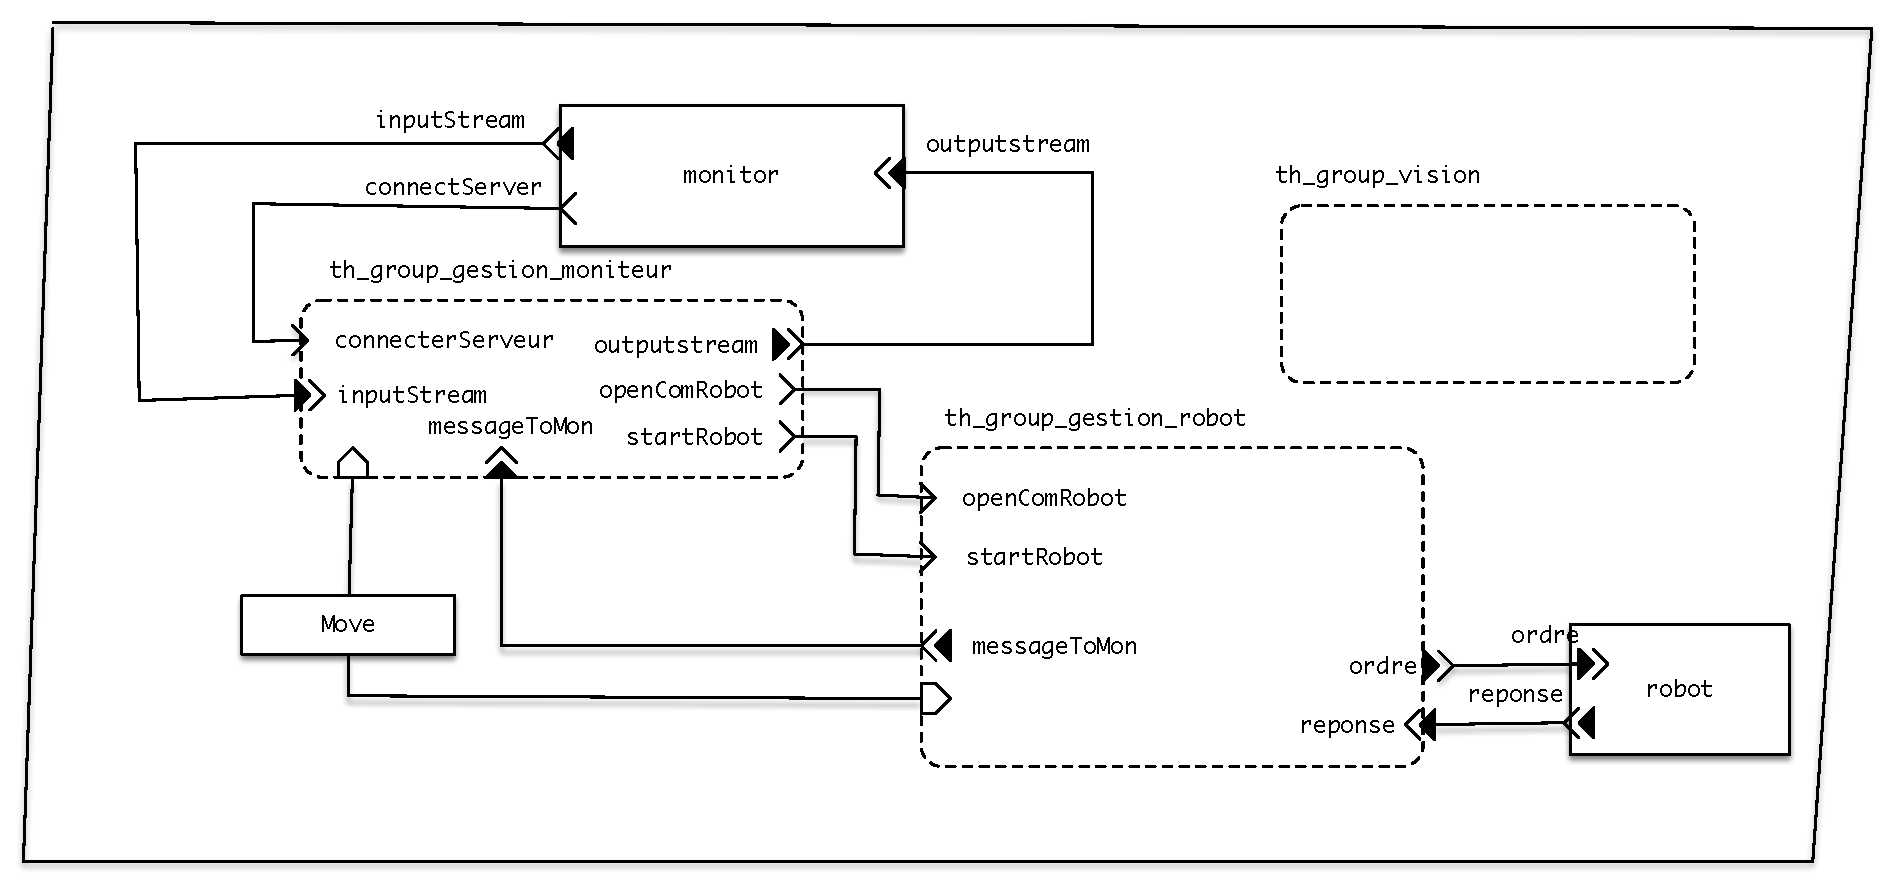
\includegraphics[scale=.5]{./figures-pdf/diag_fonc_gen}}
{\caption{Diagramme fonctionnel du système}}
\end{center}
\label{fig:diag_fonc_gen}
\end{figure}
\FloatBarrier

% DIAGRAMME FONCTIONNEL GT MONITEUR
\subsection{Groupe de threads gestion du moniteur}

{\color{red}Placez ici :
\begin{itemize}
\item le diagramme fonctionnel en AADL décrivant le groupe de threads de gestion du moniteur (voir exemple de la figure~\ref{fig:diag_fonc_moniteur} réalisée à partir du dossier de conception),
\item remplir le tableau~\ref{tab:gt_moniteur} pour expliquer le rôle de chacun des threads,
\item les diagrammes d'activité de chaque thread de ce groupe.
\end{itemize}

Décrivez tous les éléments (paramètres, variables, etc.) qui vous semblent pertinents pour comprendre les diagrammes.}

% DIAGRAMME FONCTIONNEL GT MONITEUR
\subsubsection{Diagramme fonctionnel du groupe gestion du moniteur}

{\color{red} Exemple de diagramme fonctionnel pour le groupe de thread de gestion du moniteur. Mettez à jour ce diagramme avec votre conception.}

\begin{figure}[htbp]
\label{fig:diag_fonc_moniteur}
\begin{center}
{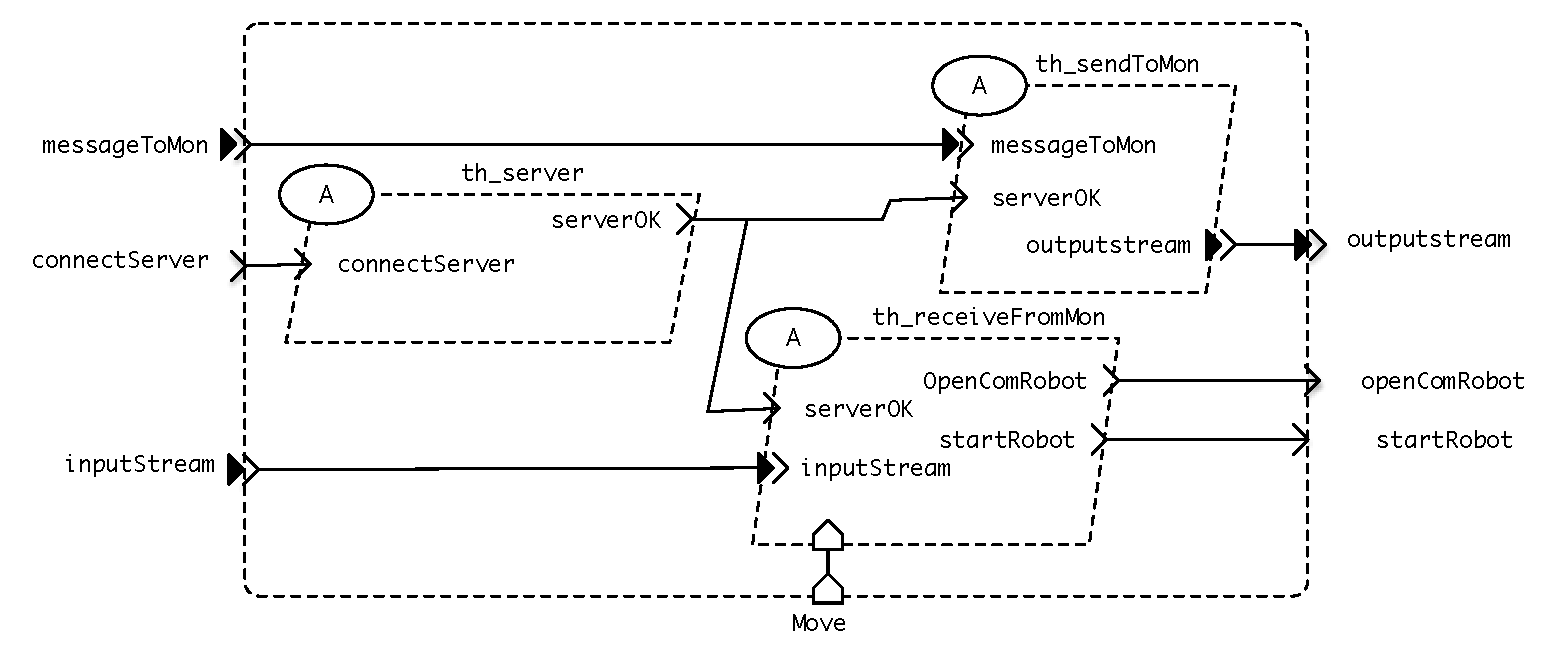
\includegraphics[scale=.5]{./figures-pdf/diag_fonc_moniteur}}
{\caption{Diagramme fonctionnel du groupe de threads gestion du moniteur}}
\end{center}
\end{figure}
\FloatBarrier

% DESCRIPTION THREADS GT MONITEUR
\subsubsection{Description des threads  du groupe gestion du moniteur}
{\color{red} Remplissez le tableau ci-dessous pour expliquer le rôle de chaque thread et donner son niveau de priorité.}


\begin{table}[htp]
\caption{Description des threads du groupe {\tt th\_group\_gestion\_moniteur}}
\begin{center}
\begin{tabular}{|p{3cm}|p{8.5cm}|p{2cm}|}
\hline
\bf Nom du thread &	\bf Rôle &	\bf Priorité \\
\hline
\hline
\color{blue}tCommuniquer	& \color{blue}Prend en charge les messages entrants depuis le moniteur & \color{blue}25\\
\hline
\color{blue}tEnvoyer	& \color{blue}Envoi l'ensemble des messages du superviseur au moniteur & \color{blue}30\\
\hline
\color{blue}... &	\color{blue}... &	\color{blue}...\\
\hline
\end{tabular}
\end{center}
\label{tab:gt_moniteur}
\end{table}%

% DIAGRAMMES D'ACTIVITE GT MONITEUR
\subsubsection{Diagrammes d'activité  du groupe gestion du moniteur}
{\color{red}Décrivez le comportement de chacun de vos threads avec des diagrammes d'activité. Apportez les explications qui vous semblent nécessaires pour comprendre votre conception. A titre d'exemple les diagrammes fonctionnels tirés du document de conception sont remis.}

\begin{figure}[htbp]
\label{fig:act_communiquer}
\begin{center}
{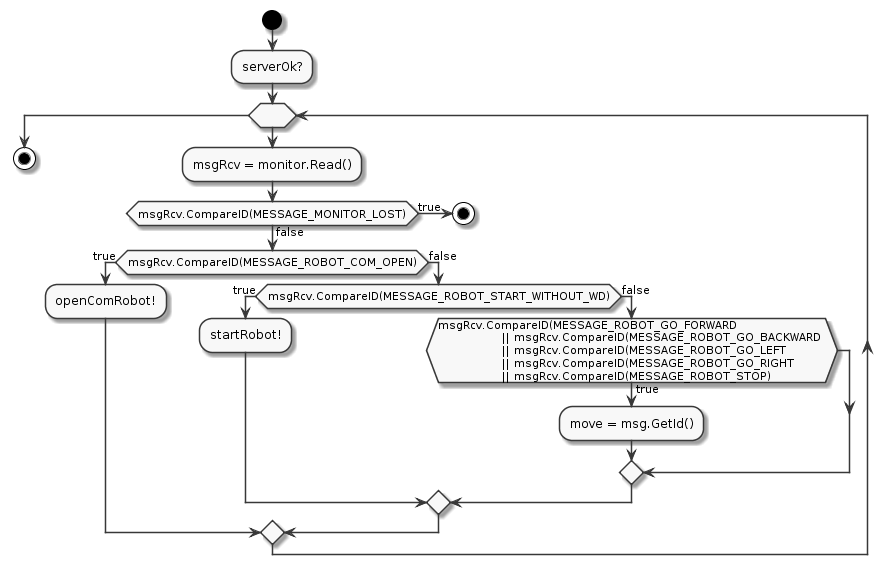
\includegraphics[scale=.3]{./figures-pdf/th_receiveFromMon.png}}
{\caption{Diagramme d'activité du thread {\tt th\_receiveFromMon}}}
\end{center}
\end{figure}


\begin{figure}[htbp]
\label{fig:act_envoyer}
\begin{center}
{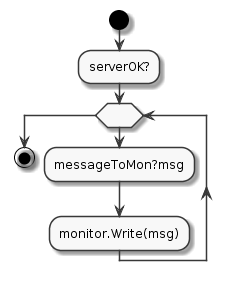
\includegraphics[scale=.3]{./figures-pdf/th_sendToMon}}
{\caption{Diagramme d'activité du thread {\tt th\_sendToMon}}}
\end{center}
\end{figure}


\begin{figure}[htbp]
\label{fig:act_envoyer}
\begin{center}
{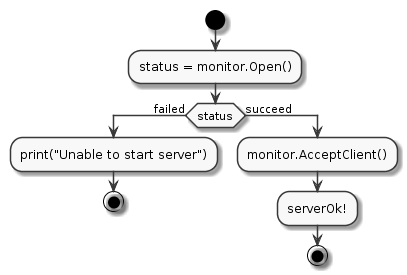
\includegraphics[scale=.3]{./figures-pdf/th_server}}
{\caption{Diagramme d'activité du thread {\tt th\_server}}}
\end{center}
\end{figure}
\FloatBarrier

% DIAGRAMME FONCTIONNEL GT VISION
\subsection{Groupe de threads vision}

% DIAGRAMME FONCTIONNEL GT VISION
\subsubsection{Diagramme fonctionnel du groupe vision}

{\color{blue} Ajoutez le diagramme fonctionnel du groupe de threads de vision.}

% DESCRIPTION THREADS GT VISION
\subsubsection{Description des threads du groupe vision}
{\color{red} Remplissez le tableau ci-dessous pour expliquer le rôle de chaque thread et donner son niveau de priorité.}


\begin{table}[htp]
\caption{Description des threads du groupe {\tt th\_group\_vision}}
\begin{center}
\begin{tabular}{|p{3cm}|p{8.5cm}|p{2cm}|}
\hline
\bf Nom du thread &	\bf Rôle &	\bf Priorité \\
\hline
\hline
\color{blue}... &	\color{blue}... &	\color{blue}...\\
\hline
\end{tabular}
\end{center}
\label{tab:gt_moniteur}
\end{table}%
\FloatBarrier

% DIAGRAMMES D'ACTIVITE GT VISION
\subsubsection{Diagrammes d'activité du groupe vision}
{\color{blue}Décrivez le comportement de chacun de vos threads avec des diagrammes d'activité. Apportez les explications qui vous semblent nécessaires pour comprendre votre conception.}


% DIAGRAMME FONCTIONNEL GT ROBOT
\subsection{Groupe de threads gestion du robot}

% DIAGRAMME FONCTIONNEL GT ROBOT
\subsubsection{Diagramme fonctionnel du groupe gestion robot}
{\color{blue} Ajoutez le diagramme fonctionnel du groupe de threads de gestion du robot.}

% DESCRIPTION THREADS GT ROBOT
\subsubsection{Description des threads du groupe gestion robot}
{\color{red} Remplissez le tableau ci-dessous pour expliquer le rôle de chaque thread et donner son niveau de priorité.}


\begin{table}[htp]
\caption{Description des threads du groupe {\tt th\_group\_gestion\_robot}}
\begin{center}
\begin{tabular}{|p{3cm}|p{8.5cm}|p{2cm}|}
\hline
\bf Nom du thread &	\bf Rôle &	\bf Priorité \\
\hline
\hline
\color{blue}... &	\color{blue}... &	\color{blue}...\\
\hline
\end{tabular}
\end{center}
\label{tab:gt_moniteur}
\end{table}%
\FloatBarrier

% DIAGRAMMES D'ACTIVITE GT ROBOT
\subsubsection{Diagrammes d'activité du groupe robot}
{\color{blue}Décrivez le comportement de chacun de vos threads avec des diagrammes d'activité. Apportez les explications qui vous semblent nécessaires pour comprendre votre conception.}


%%%%%%%%%%%%%%%
% ANALYSE ET VALIDATION
\section{Analyse et validation de la conception}

{\color{red}Pour chacune des fonctionnalités attendues, indiquez si elle a été réalisée. Ajoutez d'éventuelles remarques de conception si le fonctionnement n'est pas exactement celui attendu et justifiez le respect des propriétés temporelles. Vous n'êtes pas obligé de répondre à ces éléments pour les fonctionnalités réalisées dans la conception préliminaire (ces fonctionnalités sont indiquées dans la suite par un astérisque). Si vous ne souhaitez pas apporter de détails supplémentaires pour ces fonctionnalités, supprimez les de la liste ci-dessous.}

{\color{gray}
\stepcounter{cptreq}
\subsection{Fonctionnalité \thecptreq *}

\paragraph{Description :} Le lancement du serveur doit être réalisé au démarrage du superviseur. En cas d'échec du démarrage du serveur, un message textuel doit être  affiché sur la console de lancement de l'application. Ce message doit signaler le problème et le superviseur doit s'arrêter.

\paragraph{\color{black}Réalisation :}  {\color{blue} Fait en partie. La fonctionnalité est impléméntée sauf pour l'arrêt suite à l'échec de démarrage du serveur. L'implémentation actuelle stoppe la tâche en charge du démarrage du serveur, mais pas l'ensemble de l'application. Après discussion avec le client, la version actuelle est suffisante.}
}
%%%
{\color{gray}
\stepcounter{cptreq}
\subsection{Fonctionnalité \thecptreq *}

\paragraph{Description :} La connexion entre le moniteur et le superviseur (via le socket) doit être établie suite à la demande de connexion de l'utilisateur.

\paragraph{\color{black}Réalisation :}  {\color{red} indiquez si la fonctionnalité est traitée et s'il y a des remarques particulières.}
}

%%%
{\color{gray}
\stepcounter{cptreq}
\subsection{Fonctionnalité \thecptreq *}

\paragraph{Description :} Tous les messages envoyés depuis le moniteur doivent être réceptionnés par le superviseur.

\paragraph{\color{black}Réalisation :}  {\color{red} indiquez si la fonctionnalité est traitée et s'il y a des remarques particulières.}
%%%
\stepcounter{cptreq}
\subsection{Fonctionnalité \thecptreq *}

\paragraph{Description :} L'application superviseur doit être capable d'envoyer les messages au moniteur (via le serveur) avec un délai d'au plus 10~ms.

\paragraph{\color{black}Réalisation :}  {\color{red} indiquez si la fonctionnalité est traitée et s'il y a des remarques particulières.}
}
%%%
\stepcounter{cptreq}
\subsection{Fonctionnalité \thecptreq}

\paragraph{Description :} Le superviseur doit détecter la perte de communication avec le moniteur. En cas de perte de la communication un message doit être affiché sur la console de lancement du superviseur.

\paragraph{\color{black}Réalisation :}  {\color{red} indiquez si la fonctionnalité est traitée et s'il y a des remarques particulières.}
%%%
\stepcounter{cptreq}
\subsection{Fonctionnalité \thecptreq}

\paragraph{Description :} En cas de perte de communication entre le superviseur et moniteur, il faut stopper le robot,  la communication avec le robot, fermer le serveur et déconnecter la caméra afin de revenir dans le même état qu'au démarrage du superviseur.

\paragraph{\color{black}Réalisation :}  {\color{red} indiquez si la fonctionnalité est traitée et s'il y a des remarques particulières.}
%%%
{\color{gray}
\stepcounter{cptreq}
\subsection{Fonctionnalité \thecptreq *}

\paragraph{Description :} Dès que la communication avec le moniteur est en place, la communication entre le superviseur et le robot doit être ouverte. Si la communication est active, il faut envoyer un message d'acquittement au moniteur. En cas d'échec, un message le signalant est renvoyé au moniteur.

\paragraph{\color{black}Réalisation :}  {\color{red} indiquez si la fonctionnalité est traitée et s'il y a des remarques particulières.}
}
%%%
\stepcounter{cptreq}
\subsection{Fonctionnalité \thecptreq}

\paragraph{Description :} La communication entre le robot et le superviseur doit être surveillée par un mécanisme de compteur afin de détecter une perte du médium de communication.

\paragraph{\color{black}Réalisation :}  {\color{red} indiquez si la fonctionnalité est traitée et s'il y a des remarques particulières.}

%%%
\stepcounter{cptreq}
\subsection{Fonctionnalité \thecptreq}

\paragraph{Description :} Lorsque la communication entre le robot et le superviseur est perdue, un message spécifique doit être envoyé au moniteur. Le système doit fermer la communication entre le robot et le superviseur et se remettre dans un état initial permettant de relancer la communication.

\paragraph{\color{black}Réalisation :}  {\color{red} indiquez si la fonctionnalité est traitée et s'il y a des remarques particulières.}

%%%
{\color{gray}
\stepcounter{cptreq}
\subsection{Fonctionnalité \thecptreq *}

\paragraph{Description :} Lorsque l'utilisateur demande, via le moniteur, le démarrage sans watchdog, le robot doit démarrer dans ce mode. En cas de succès, un message d'acquittement est retourné au moniteur. En cas d'échec, un message indiquant l'échec est transmis au moniteur.

\paragraph{\color{black}Réalisation :}  {\color{red} indiquez si la fonctionnalité est traitée et s'il y a des remarques particulières.}
}
%%%
\stepcounter{cptreq}
\subsection{Fonctionnalité \thecptreq}

\paragraph{Description :} Lorsque l'utilisateur demande, via le moniteur, le démarrage avec watchdog, le robot doit démarrer dans ce mode. Un message d'acquittement est retourné au moniteur. En cas d'échec, un message indiquant l'échec est transmis au moniteur.

Une fois le démarrage effectué, le robot doit rester vivant en envoyant régulièrement le message de rechargement du watchdog.

\paragraph{\color{black}Réalisation :}  {\color{red} indiquez si la fonctionnalité est traitée et s'il y a des remarques particulières.}

%%%
{\color{gray}
\stepcounter{cptreq}
\subsection{Fonctionnalité \thecptreq *}

\paragraph{Description :} Lorsque qu'un ordre de mouvement est reçu par le superviseur, le robot doit réaliser ce déplacement en moins de 100~ms.

\paragraph{\color{black}Réalisation :}  {\color{blue} Cette fonctionnalité a été implémentée à l'aide d'une tâche qui envoie toutes les 100~ms un ordre de mouvement au robot une fois que celui-ci est démarré (tâche th\_move). Cette implémentation ne garantit pas que le temps soit inférieur à 100~ms entre la réception du message et sa prise en compte par le robot. En effet, le temps de traitement de la réception par la tâche th\_receiveFromMon, le temps de traitement de la tâche th\_move et celui de l'envoi de l'ordre via le Xbee ne sont pas considérés. Afin de réduire ces délais, les priorités de  th\_receiveFromMon et de th\_move sont élevés mais ne permettent pas de garantir l'exigence de temps. Augmenter la fréquence de la tâche th\_move permettrait de tenir cette contrainte, mais risque de surcharger la communication avec le robot (une version avec l'envoi de l'ordre que s'il a changé serait souhaitable). Finalement, une version asynchrone (attente d'un événement-donnée entre th\_receiveFromMon et de th\_move) aurait été préférable. Cependant, après discussion avec le client, la version périodique à 100~ms est cependant validée.}
}
%%%
\stepcounter{cptreq}
\subsection{Fonctionnalité \thecptreq}

\paragraph{Description :} Le niveau de la batterie du robot doit être mis à jour toutes les 500~ms sur le moniteur.

\paragraph{\color{black}Réalisation :}  {\color{red} indiquez si la fonctionnalité est traitée et s'il y a des remarques particulières.}
%%%
\stepcounter{cptreq}
\subsection{Fonctionnalité \thecptreq}

\paragraph{Description :} La caméra doit être démarrée suite à une demande provenant du moniteur. Si l'ouverture de la  caméra a échoué, il faut envoyer un message au moniteur.

\paragraph{\color{black}Réalisation :}  {\color{red} indiquez si la fonctionnalité est traitée et s'il y a des remarques particulières.}
%%%
\stepcounter{cptreq}
\subsection{Fonctionnalité \thecptreq}

\paragraph{Description :} Dès que la caméra est ouverte, une image doit être envoyée au moniteur toutes les 100 ms.

\paragraph{\color{black}Réalisation :}  {\color{red} indiquez si la fonctionnalité est traitée et s'il y a des remarques particulières.}
%%%
\stepcounter{cptreq}
\subsection{Fonctionnalité \thecptreq}

\paragraph{Description :} La caméra doit être fermée suite à une demande provenant du moniteur. Un message doit être envoyé au moniteur pour signifier l'acquittement de la demande. L'envoi périodique des images doit alors être stoppé.

\paragraph{\color{black}Réalisation :}  {\color{red} indiquez si la fonctionnalité est traitée et s'il y a des remarques particulières.}
%%%
\stepcounter{cptreq}
\subsection{Fonctionnalité \thecptreq}

\paragraph{Description :} Suite à une demande de recherche de l'arène, le superviseur doit stopper l'envoi périodique des images, faire la recherche de l'arène et renvoyer une image sur laquelle est dessinée cette arène. Si aucune arène n'est trouvée un message d'échec est envoyé.\\

L'utilisateur doit ensuite valider visuellement via le moniteur si l'arène a bien été trouvée. L'utilisateur peut :
\begin{itemize}
	\item valider l'arène : dans ce cas, le superviseur doit sauvegarder l'arène trouvée (pour l'utiliser ultérieurement) puis retourner dans son mode d'envoi périodique des images en ajoutant à l'image l'arène dessinée.
 	\item annuler la recherche : dans ce cas, le superviseur doit simplement retourner dans son mode d'envoi périodique des images et invalider la recherche.
\end{itemize}

\paragraph{\color{black}Réalisation :}  {\color{red} indiquez si la fonctionnalité est traitée et s'il y a des remarques particulières.}
%%%
\stepcounter{cptreq}
\subsection{Fonctionnalité \thecptreq}

\paragraph{Description :} Suite à une demande de l'utilisateur de calculer la position du robot, le superviseur doit calculer cette position, dessiner sur l'image le résultat et envoyer un message au moniteur avec la position toutes les 100~ms. Si le robot n'a pas été trouvé, un message de position est envoyé avec une position (-1,-1).

\paragraph{\color{black}Réalisation :}  {\color{red} indiquez si la fonctionnalité est traitée et s'il y a des remarques particulières.}
\stepcounter{cptreq}
\subsection{Fonctionnalité \thecptreq}

\paragraph{Description :} Suite à une demande de l'utilisateur de stopper le calcul de la position du robot, le superviseur doit rebasculer dans un mode d'envoi de l'image sans le calcul de la position.

\paragraph{\color{black}Réalisation :}  {\color{red} indiquez si la fonctionnalité est traitée et s'il y a des remarques particulières.}


%%%%%%%%%%%%%%%%%%%
% TRANSFORMATION AADL2XENO
\section{Transformation AADL vers Xenomai}
 
 {\color{red} Cette section est consacrée à la méthode pour passer d'un modèle AADL à un code sous Xenomai. Pour chacun des éléments AADL, vous expliquerez {\bf comment vous l'avez traduit en code} et quels {\bf services de Xenomai} vous avez utilisés {\bf en expliquant ce qu'ils font}. Chaque élément devra être illustré avec des {\bf extraits de code de votre projet}.}
 
 % THREAD
\subsection{Thread}
% INSTANCIATION THREAD
\subsubsection{Instanciation et démarrage}
 {\color{blue} Expliquer comment vous implémentez sous Xenomai l'instanciation et le démarrage d'un  thread AADL.}
 
 {\color{blue} {\bf Exemple de réponse} : Chaque thread a été implémenté par un {\tt RT\_TASK} déclarés dans le fichier {\tt tasks.h}. La création de la tâche se fait à l'aide du service {\tt rt\_task\_create} et son démarrage à l'aide de {\tt rt\_task\_start}. Toutes les tâches sont crées dans la méthode {\tt init} de {\tt tasks.cpp} et démarrées dans la méthode {\tt run}.

Par exemple, pour la tâche {\tt th\_server}, sa déclaration est faite ligne 73 dans le fichier {\tt tasks.h}
\begin{verbatim}
  RT_TASK th_server;
\end{verbatim}
sa création ligne 102 de {\tt tasks.cpp} lors de l'appel de
\begin{verbatim}
  rt_task_create(&th_server, "th_server", 0, PRIORITY_TSERVER, 0)
\end{verbatim}
et son démarrage ligne 146 avec
\begin{verbatim}
  rt_task_start(&th_server, (void(*)(void*)) & Tasks::ServerTask, this)
\end{verbatim}
}

% CODE THREAD
\subsubsection{Code à exécuter}
 {\color{blue} Comment se fait le lien sous Xenomai entre le thread et le traitement à exécuter.}

% PRIORITE THREAD
\subsubsection{Niveau de priorités}
 {\color{blue} Expliquer comment vous fixez sous Xenomai le niveau de priorité d'un thread AADL.}

% PERIODICITE THREAD
\subsubsection{Activation périodique}
 {\color{blue} Expliquer comment vous rendez périodique l'activation d'un thread AADL sous Xenomai.}

% THREAD EVENEMENTIEL
\subsubsection{Activation événementielle}
 {\color{blue} Expliquer les moyens mis en {\oe}uvre dans l'implémentation sous Xenomai pour gérer les activations événementielles d'un thread AADL.}

 
 % PORT D'EVENEMENT
\subsection{Port d’événement}

% INSTANCIATION PORT D'EVENEMENT
\subsubsection{Instanciation}
 {\color{blue} Comment avez-vous instancié un port d'événement ?}\\
 
 % ENVOI PORT D'EVENEMENT
\subsubsection{Envoi d’un événement}
 {\color{blue} Quels services ont été employés pour signaler un événement ?}

% RECEPTION PORT D'EVENEMENT
\subsubsection{Réception d’un événement}
 {\color{blue} Comment se fait l'attente d'un événement ?}

% DONNEE PARTAGEE
\subsection{Donnée partagée}

% INSTANCIATION DONNEE PARTAGEE
\subsubsection{Instanciation}
 {\color{blue} Quelle structure instancie une donnée partagée ?}

% LECTURE/ECRITURE DONNEE PARTAGEE
\subsubsection{Accès en lecture et écriture}
 {\color{blue} Comment garantissez-vous sous Xenomai l'accès à une donnée partagée ?}

% PORT D'EVENEMENT-DONNEES
\subsection{Ports d’événement-données}

% INSTANCIATION PORT D'EVENEMENT-DONNEES
\subsubsection{Instanciation}
 {\color{blue} Donnez la solution retenue pour implémenter un port d'événement-données avec Xenomai.}

% ENVOI PORT D'EVENEMENT-DONNEES
\subsubsection{Envoi d’une donnée}
 {\color{blue} Quels services avez-vous employés pour envoyer des données ?}

% RECEPTION PORT D'EVENEMENT-DONNEES
\subsubsection{Réception d’une donnée}
 {\color{blue} Quels services avez-vous employés pour recevoir des données ?}
 




\end{document}